\documentclass[sigchi, anonymous=true]{acmart}

\usepackage{booktabs} % For formal tables
\usepackage{adjustbox}
\usepackage{refcount}
\usepackage{colortbl}
\usepackage{graphicx,subcaption}
\usepackage{listings}

% Copyright
%\setcopyright{none}
%\setcopyright{acmcopyright}
\setcopyright{acmlicensed}
%\setcopyright{rightsretained}
%\setcopyright{usgov}
%\setcopyright{usgovmixed}
%\setcopyright{cagov}
%\setcopyright{licensedcagov}
%\setcopyright{cagovmixed}
%\setcopyright{licensedothergov}

% DOI
% \acmDOI{10.475/123_4}

% ISBN
% \acmISBN{123-4567-24-567/08/06}

%Conference
\acmConference[ETRA'19]{ACM ETRA conference}{June 2019}{Denver, Colorado USA}
\acmYear{2019}
\copyrightyear{2018}

\acmPrice{15.00}


\begin{document}
% \title{Power-efficient and Robust to Shifts Photo-oculography-based Eye-tracking Sensors}
\title{Power-efficient and shift-robust eye-tracking sensor for portable VR headsets}
%\titlenote{Produces the permission block, and
%  copyright information}
%\subtitle{Extended Abstract}
%\subtitlenote{The full version of the author's guide is available as
%  \texttt{acmart.pdf} document}

\author{Dmytro Katrychuk}
\affiliation{%
  \institution{Department of Computer Science, Texas State University}
  \streetaddress{Derrick Hall M5, 601 University
Drive}
  \city{San Marcos}
  \state{Texas}
  \postcode{78666}
}
\email{d_k139@txstate.edu}
\author{Henry K. Griffith}
\affiliation{%
  \institution{Department of Computer Science, Texas State University}
  \streetaddress{Derrick Hall M5, 601 University
Drive}
  \city{San Marcos}
  \state{Texas}
  \postcode{78666}
}
\email{h_g169@txstate.edu}
\author{Oleg V. Komogortsev}
\affiliation{%
  \institution{Department of Computer Science, Texas State University}
  \streetaddress{Derrick Hall M5, 601 University
Drive}
  \city{San Marcos}
  \state{Texas}
  \postcode{78666}
}
\email{ok@txstate.edu}
% \authornote{Dr.~Trovato insisted his name be first.}
% \orcid{1234-5678-9012}



% \authornote{The secretary disavows any knowledge of this author's actions.}
% \affiliation{%
%   \institution{Department of Computer Science, Texas State University}
%   \streetaddress{Comal Building 307D, 601 University
% Drive}
%   \city{San Marcos}
%   \state{Texas}
%   \postcode{78666}
% }
% \email{ok@txstate.edu}

% The default list of authors is too long for headers.
\renewcommand{\shortauthors}{Katrychuk et al.}


\begin{abstract}
% Video oculography (VOG) is the most common method of eye tracking today. Due to VOG' high power consumption its usage is mostly restricted to wired solutions. However, headset mobility is important for many virtual reality (VR) applications. This paper pushes forward development and validation of photosensor oculography (PS-OG), an alternative eye-tracking technique that targets to enable low cost and low power eye-tracking in any portable VR headset. Its main drawback lies in drastic spatial accuracy degradation with even slight sensor shifts. In this work we employ machine learning to build a mapping between raw sensor outputs and eye gaze position to make PS-OG tolerant to shifts. We consider various neural network architectures and approaches to train them while restricting power consumption to meet the limitations of the embedded hardware. The results indicate that it is possible to achieve spatial accuracy on par with existing VOG solutions. Further evaluation without strict power limitations shows the potential of the proposed technology to replace current solutions---even wired setups---due to better spatial accuracy, higher sampling frequency and reduced overall power consumption.
Current eye-tracking systems mainly employ video oculography. Due to the high power consumption of this approach, its usage is restricted to wired solutions; but mobility is important for many virtual reality (VR) applications. This paper validates photosensor oculography, an alternative eye-tracking technique that may enable eye-tracking in any portable VR headset. Its main drawback lies in drastic accuracy degradation with even slight sensor shifts. Applying machine learning to build a mapping between raw sensor outputs and eye gaze position helps to mitigate this problem. Various neural networks and approaches to train them are evaluated while restricting power consumption to meet the limitations of embedded hardware. Our results report spatial accuracy on par with existing video oculography solutions. Further evaluation without strict power limitations shows the potential of the proposed technology to replace current solutions---even wired setups---due to better accuracy and higher sampling frequency available.
\end{abstract}

%
% The code below should be generated by the tool at
% http://dl.acm.org/ccs.cfm
% Please copy and paste the code instead of the example below.
%
\begin{CCSXML}
<ccs2012>
<concept>
<concept_id>10003120.10003121.10003124.10010866</concept_id>
<concept_desc>Human-centered computing~Virtual reality</concept_desc>
<concept_significance>500</concept_significance>
</concept>
<concept>
<concept_id>10010583.10010662.10010674</concept_id>
<concept_desc>Hardware~Power estimation and optimization</concept_desc>
<concept_significance>300</concept_significance>
</concept>
<concept>
<concept_id>10010583.10010717.10010721.10010725</concept_id>
<concept_desc>Hardware~Simulation and emulation</concept_desc>
<concept_significance>300</concept_significance>
</concept>
</ccs2012>
\end{CCSXML}

\ccsdesc[500]{Human-centered computing~Virtual reality}
\ccsdesc[300]{Hardware~Power estimation and optimization}
\ccsdesc[300]{Hardware~Simulation and emulation}


\keywords{eye-tracking, virtual reality, VR, photo-sensor oculography, PSOG, machine learning, ML}

\maketitle

\section{Introduction}\label{sec:intro}

Evidenced by increasing adoption within commercial headsets, eye-tracking (ET) technology offers notable potential for improving the user-experience in virtual and augmented reality (VR/AR) environments. The visual system is one of our main tools for interacting with the surrounding environment, so ET empowers a natural dimension of human computer interaction (HCI). This capability is crucial to provide accessibility for disabled individuals who are unable to use traditional input modalities. Real-time ET may also be used to deploy foveated rendering which produces high-quality content only near the point of gaze  ~\cite{guenter2012foveated}. This strategy can decrease power consumption or preserve the same amount of it but improve the rendering quality.

The specific traits of each subject's oculomotor system, eye shape, periocular features etc., were proved to have great potential for biometrics and health assessment applications. In the lab environment, it is possible to build a biometrics system with an equal-error rate (EER) of less than $3$\% which is on par with a fingerprint sensor \cite{friedman2017method}. The main advantage of such a system is that there is no known way to spoof it, which is not the case for a fingerprint sensor or facial recognition system. With respect to health assessment, the detection of various diseases and states, including schizophrenia, mild traumatic brain injury, intoxication and fatigue , have been demonstrated using eye movement signals.

ET sensors in current VR headsets utilize video-based oculography (VOG) technology. VOG illuminates the eye using a set of infrared (IR) emitters, captures reflections using an IR camera, and estimates gaze location using image processing techniques. VOG sensors offer a robust, non-invasive ET solution, and are integrated within the majority of stand-alone ET devices. High-quality VOG systems for laboratory use may be engineered to achieve tremendous performance, including sampling rates up to $2000 Hz$, along with spatial accuracy and precision scores of less than $0.5$\textdegree{} and $0.05$\textdegree{} of the visual angle, respectively  (EyeLink 1000 Plus, \cite{EyeLink1000P}). VOG sensors within current VR headsets, such as FOVE VR and HTC Vive with third-party add-ons from SMI or PupilLabs, are restricted in sampling rate to $250 Hz$, and have less than $1.0$\textdegree{} spatial accuracy. Moreover, requirements of form factor and available processing power, prohibits using VOG in wireless headsets like Google Daydream or Samsung Gear VR.

Photosensor oculography (PSOG) ~\cite{torok1951lxxx} offers a promising solution for addressing the aforementioned limitations of VOG devices.  By capturing the IR reflection from the eye using only a sparse grid of IR detectors, PSOG dramatically reduces computational requirements and promotes increased sampling rate. Unfortunately, the performance sensitivity of PSOG devices to sensors shift poses new challenges. As mentioned in ~\cite{rigas2017hybrid}, the shift of more than $0.5mm$ result in more than $1.0$\textdegree{} spatial accuracy degradation. Usual VR applications, such as gaming, social interaction or learning in a simulated environment, will not be possible without changing facial expressions, repositioning the head, or moving freely. During any of these activities, slight headset shifts are likely to occur, so viable ET solutions must exhibit robustness to sensors shift.

This study advances the development of shift-robust PSOG ET sensors with accuracy on par with existing VOG solutions for wired VR headsets. We expand the literature by evaluation of a convolutional-neural-network (CNN) utilized together with transfer learning to build a calibration mapping in the presence of simulated sensor shifts. Moreover, our work improves upon previous studies based on synthetic data by using actual eye images of multiple subjects obtained from a custom eye-tracker.    

\section{Prior work}

PSOG estimates gaze location using a signal captured from a sparse array of IR receiving sensors. Reflections are induced through active illumination by IR emitters.  PSOG exploits the varying IR reflectivity of different components of the eye, such as the pupil, iris, sclera, etc. As the eye rotates within the globe during gaze shifts, intensities of reflections captured by IR sensors are perturbed, thereby providing the source for estimating gaze location. PSOG designs are distinguished according to both physical parameters of the IR transceiver hardware, along with the signal processing techniques used to map sensors output to the estimated gaze location. For purposes of our current work, we focus solely on signal mapping techniques, using sensors placement developed in previous studies. The recent review of the various PSOG designs can be found in \cite{rigas2018photosensor}. This section is restricted to describing the limitations of two recent publications which have motivated our current work.

While PSOG offers a promising alternative for meeting the performance requirements of next-generation VR solutions, sensitivity to hardware shifts limits practical viability. Two recent approaches have been proposed to address this limitation. Rigas et al. suggested a fused sensing modality known as Hybrid PS-V  \cite{rigas2017hybrid}. In this approach, gaze estimates formed using a high-speed ($1000 Hz$) PSOG component are fused with low-speed VOG ($5Hz$) sensor output to improve spatial accuracy in the presence of sensor shifts. The authors simulated a $2x2$ grid of IR receivers using reflectivity estimates obtained from synthetic images of a close eye region. Eye position was inferred from simulated PSOG outputs by a simple deterministic mapping. Due to the decreased VOG sampling rate, the proposed architecture was estimated to consume only $15 mW$ of power, a reduction of several orders of magnitude versus commercially-available VOG-only systems operating at the same sampling frequency (e.g. EyeLink 1000). Spatial accuracy of less than $1.0$\textdegree{} of the visual angle was achieved in the presence of sensor shifts in the range of $\pm 2mm$. The main drawbacks of this approach are brief spike artifacts in the output eye signal during sensor movement phase and up to $200 ms$ latency of the correction system. Additionally, the reliance upon an additional tracking modality may prove infeasible for resource-constrained environments. Finally, the work uses synthetically generated eye images for a single artificial subject, which greatly inhibits inference regarding generalization.

To eliminate the VOG requirement, Zemblys et al. utilized machine learning to achieve shift-robustness \cite{zemblys2018making}. MLP was used to build the mapping between the PSOG output and gaze location. Model hyper-parameters were determined empirically using a standard grid-search procedure. The authors evaluated different sensor placements and found that $3x5$ rectangular grid works best. The best setup found has spatial accuracy of $0.48$\textdegree{} of the visual angle for sensor shifts in the range of $\pm 1.75mm$. However, it is characterized by the same limitations of the previous work with respect to the utilization of a single-model synthetic data source. It is still not clear how well those approaches will work when applied to real images and diverse eye traits. Moreover, the machine learning models explored are not well-suited to capture the inherent spatial dependencies of PSOG outputs, compared to the convolutional architectures considered herein. 

Our work addresses the limitations of these two studies by considering more advanced machine learning techniques on data gathered from real recordings of different subjects.

\section{Methodology}

\subsection{Equipment}

A custom ET solution introduced in \cite{abdulin2017study})  was used for data collection. This system was used in place of standard commercial solutions, such as EyeLink 1000, due to the failure of that equipment to save images obtained by the VOG sensor. The custom solution  offers an additional advantage in a research environment, as it is highly reconfigurable (i.e.: easily replaceable IR emitters, camera, and chin-rest) and uses open-source software. To collect data used in this work, the system uses an 850 nm IR illuminator, ThorLabs DCC1545M camera,  and a hot mirror and chin-rest from EyeLink 1000. The camera recorded monocular images with a resolution of $348x640$ pixels at $120$ fps. 
A random saccade stimulus was displayed on a screen installed $500mm$ away from the chin-rest . The display has a resolution of $1280x1024$,  and physical size of $374x300 mm$, affording a target range of $\pm 19.1$\textdegree{} (horizontal)  and $\pm 16.7$\textdegree{} (vertical) degrees of visual angle. All computations were performed using a workstation with the following specifications: Intel Core i7-6700K CPU, 16GB RAM, Nvidia GTX 970 GPU.

\subsection{Data}

\begin{figure}[h]
\begin{center}
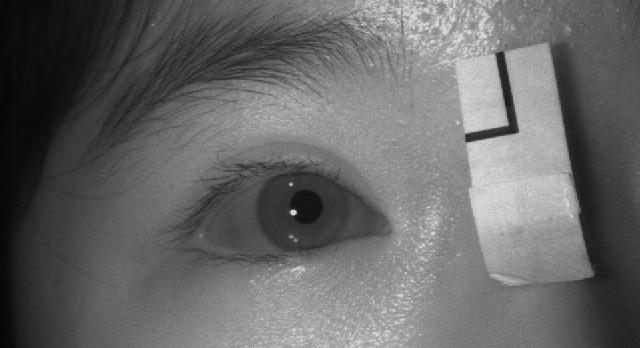
\includegraphics[width=0.35\textwidth]{data_frame.jpg}
\end{center}
   \caption{One IR frame from the data set}
\label{fig:data_frame}
\end{figure}

Data was collected for 23 subjects. Every subject's record consists of the set of images and respective eye-movement signal file. Each line of this file contains a timestamp, and corresponding horizontal and vertical gaze estimates expressed in degrees of the visual angle. If for some reason eye-tracker was not able to infer eye gaze at the specific timestamp, (i.e: during blinks, etc.), the corresponding line is filled with $NaN$s. Moreover, by inspecting frequency histograms of eye gaze positions, it was detected that sometimes eye-tracker reports values far outside of the screen range (probably, just before or right after a blink). To account for that, every eye gaze position outside of the $\pm20$\textdegree{} range either horizontally or vertically is filtered out.    

As shown in Figure \ref{fig:data_frame}, an angular marker was attached to each subject's nasal bone area in order to account for slight head movements during recording as described below. This approach was unsuccessful for Subject 9, resulting in removal from the data set. 

\subsection{Preprocessing}

To begin preprocessing, potential head-movements were estimated by tracking the position of the angular marker throughout each image sequence on a per-subject basis. The marker's position was manually found in the first frame. Then, the location of it was updated by searching in a nearby region centered around the previous point. This estimated shift is hereby denoted as $\Delta head$. 

In prior work using synthetic eye images, sensor shifts were simulated by moving the position of a virtual camera within Blender. As our data was collected using a real IR camera with a fixed position, this approach was not possible. To simulate shifting, a cropping strategy was employed on the captured image as follows. By taking a picture of a ruler it was determined that $0.5mm$ corresponds to about 4 pixel shift for our hardware setup. In this study, we test the range of $\pm 2mm$ shift with $0.5$ mm step which results in $\pm 16$ pixels shift with 4 pixels step. Let $\Delta cam$ denote the simulated shift. Then for each image, the top-left corner of a cropping rectangle is positioned at $start + \Delta head + \Delta cam$, where $start$ is determined manually for each recording so that for no shift case the eye in the cropped image will be centered by width and it will be enough pixels in the original image to crop by height. 

PSOG output is simulated using the exact same approach as in ~\cite{zemblys2018making}. The sensor simulated by a set of receptive windows aligned in a $3x5$ rectangular grid. Each window consists of $121x121$ pixels , with mirror padding employed if it runs out of the image. To reflect the angular reception loss observed in a photosensor, each window is convolved with a Gaussian kernel with $0$ mean and $1/4$ of the window size as standard deviation. The average pixel intensity over the whole window after convolution is considered as the corresponding photosensor's raw output. 

The entire preprocessing pipeline is depicted in Figure ~\ref{fig:data_preproc}.

% Each video was frame-by-frame split to the set of images. Then all images are cropped in a certain way to a close eye-region capture. The final goal is robust-to-shifts eye-tracker so our data should contain images taken from slightly different positions. In the previous studies ~\cite{rigas2017hybrid}, ~\cite{zemblys2018making}, when Blender simulation is used, it was possible to achieve this by changing a virtual camera position. Unfortunately, it's not possible in our case, because the camera in the eye-tracker setup was sturdily fixed. We decided to simulate this sensor shifts by cropping different regions of the original image so eye in the resulting image will change its location. The big source of such change that is inherent to this data is subjects head movements during a recording, so to get controlled range of shifts we need to account for them. To achieve it, on the first image of each recording the bottom-right corner of black angular marker was manually determined. Then for each pair of consecutive images $15x15$ pixels window with the center in the previous corner position is inspected. Each pixel from this window considered as the center of $?x?$ region euclidean distance between which and the $?x?$ pattern taken from previous image with the center in the corner position is calculated, The point that is the center of the region with the smallest euclidean distance is considered as the new corner position. Let the difference between new and previous corner position be $\Delta head$. By taking a picture of a ruler it was determined that $0.5mm$ corresponds to about 4 pixel shift for our hardware setup. In this study we test the range of $\pm 2mm$ shift with $0.5$ mm step which results in $\pm 16$ pixels shift with 4 pixels step. Let the simulated shift be $\Delta cam$. Then for each image the top-left corner of cropping rectangle is determined by $start + \Delta head + \Delta cam$, where $start$ is determined manually for each recording in such way that for no shift case the eye in the cropped image will be centered by width and it will be enough pixels in the original image to crop by height.

% To simulate PSOG sensors output exactly the same approach as in ~\cite{zemblys2018making} is used. Centers of receptive windows are aligned in $3x5$ rectangular grid. To reflect the angular reception loss observed in a photosensor, each window is convolved with Gaussian kernel with $0$ mean and $1/4$ of window size as standard deviation. The average pixel intensity over the whole window after the convolution is considered as the corresponding photosensors raw output. Zemblys et al. used $121$ pixels as the window size and the mirror padding if a window runs out of an image.

% The whole preprocessing pipeline can be seen at Figure ~\ref{fig:data_preproc}

% The approach proposed to account for head movements wasn't successful for subject 9 and he(?) was removed from the data set.

\subsection{Machine learning}\label{ssec:ml}

The prior machine learning study used a multilayer perceptron (MLP) model to learn the mapping from raw photosensor outputs to eye gaze position. The two-dimensional array of outputs (in our case, $3x5$) is flattened to a one-dimensional vector to form the MLP input. This representation does not preserve spatial information, which may limit the power of this approach. CNN is a natural solution for addressing this limitation, as spatial information is maintained throughout the initial convolutional layers. For comparison purposes, we benchmark a CNN model against a comparable MLP architecture.  

In practice, the amount of training data available will be restricted to what can be obtained during calibration, which may limit the performance of the learned map. To expand the pool of available training data, we propose a transfer learning approach, where network weights are initialized through training over a large pool of other subjects. We hope that this approach (hereby denoted as the "fine-tune" approach) will allow layers of the pre-trained network to learn features that are general for eye movements across subjects. By fine-tuning this model for the specific subject using calibration data, we expect faster convergence and improved accuracy versus training using randomly initialized weights (hereby denoted as the "from-scratch" approach). Note that for both architectures only fully-connected layers were fine-tuned .

We use data whitening followed by PCA that keeps components which explain more than $99$\% of variance for MLP architecture. To preserve spatial information, only data whitening is used for CNN architecture.  

To assess the validity of the fine-tune approach, we partitioned available data into testing and training sets using an idea similar to k-fold cross-validation. Namely, the whole set is split into following 6 batches (subject's ids are listed): $[1,2,3,4]$; $[5,6,7,8]$; $[10,11,12,13]$; $[14,15,16,17]$; \\ $[18,19,20]$; $[21,22,23]$;. Then, each batch is separately considered as a testing set, with the remaining batches used for training and validation purposes. For the "from-scratch" approach, testing and training sets are obtained by partitioning data for each individual subject 

Hyper-parameters for both MLP and CNN architectures were determined using a grid search approach. Two setups  were investigated reflecting the varying use-cases of the sensor. Namely, while we are most interested in embedded VR applications, we also seek to investigate unconstrained performance for stand-alone implementations. We hereby denote these two scenarios of interest as low-power and high-power setup, respectively. 

According to \cite{bengio2012practical}, a network with the same size of layers   shows comparable performance to the case of a network with layers of varying size  but the same overall number of parameters. We use this finding to simplify the grid search procedure. Instead of having a separate number of neurons for each fully-connected layer or number of filters for each convolution layer  , we can describe the whole MLP network with two parameters: $L - $ number of layers with $N$ neurons in each; and the whole CNN network with four values: $L_{conv} - $ number of convolution layers, each of depth $D$, $L_{fc} - $ number of fully-connected layers with $N$ neurons in each. Note that for all CNN layers, a $3x3$ kernel size with a stride of $1$ is used, with a zero padding to preserve filters size ('same' in Keras terms). The same designations and assumptions about a convolutional layer will be used throughout this section. Each combination of parameters listed below composes the preliminary grid search space for the specific setup:

\begin{itemize}

    \begin{minipage}{0.90\columnwidth}
    \item Low-power setup, MLP architecture:
    \begin{lstlisting}[mathescape]
$L$ from [3,4,5,6]:
  $N$ from [16,20,24,28,32]
    \end{lstlisting}
    \end{minipage}
    
    \begin{minipage}{0.90\columnwidth}
    \item Low-power setup, CNN architecture:
    \begin{lstlisting}[mathescape]
$L_{conv}$ from [1,2,4]:
  $D$ from [4,8,16]:
    $L_{fc}$ from [3,4,5,6]:
      $N$ from [16,20,24,28,32]
    \end{lstlisting}
    \end{minipage}
    
    \begin{minipage}{0.90\columnwidth}
    \item High-power setup, MLP architecture:
    \begin{lstlisting}[mathescape]
$L$ from [3,4,5,6]:
  $N$ from [16,32,48,64,96,128]
    \end{lstlisting}
    \end{minipage}
    
    \begin{minipage}{0.90\columnwidth}
    \item High-power setup, CNN architecture:
    \begin{lstlisting}[mathescape]
$L_{conv}$ from [1,2,4]:
  $D$ from [4,8,16]:
    $L_{fc}$ from [3,4,5,6]:
      $N$ from [16,32,48,64,96,128]
    \end{lstlisting}
    \end{minipage}

\end{itemize}

The number of operations performed during the inference directly influences the power consumption of the system. As an additional restriction, the upper-limit for architecture complexity was set in accordance to resources available on the destination hardware. We use the same estimation of the power consumption of a neural network, as in \cite{zemblys2018making} - the number of floating point operations per second (FLOPS) needed to do the forward pass. Multiplications only are taken into account. We use following formulas to approximate FLOPS complexity for:

\begin{itemize}
    \item MLP architecture: \begin{equation}\begin{split}
        MLP_{flops} = f(1, n_{in}, n) + f(n_{in}, n_1, n_2) + ... + \\ f(n_{L-1}, n_L, n_{out})
    \end{split}\end{equation} where $n_i - $ number of neurons in $i$-th layer, \\ $(n_{in}, 1), (n_{out}, 1)$ - dimensions of the input and output vectors respectively, and:
    \[f(x, y, z) = 2xyz - xz\]
    In our case, when the size of the input vector depends on the PCA result, the number of neurons $n$ is the same for all layers and $L > 2$, this simplifies to:
    \begin{equation}\begin{split}
        MLP_{flops} = f(1, n_{PCA}, n) + f(n_{PCA}, n, n) + \\ (L - 2)*f(n, n, n) + f(n, n, 2)\label{eq:1}\end{split}
        \end{equation}
    \item CNN architecture: \begin{equation}\begin{split}
        CNN_{flops} = m*(1 + D_1 + ... + D_{L_{conv}-1})\, + \\ f(1, n_{flatten}, n_1) + f(n_{flatten}, n_1, n_2) + ... + \\ f(n_{L_{fc}-1}, n_{L_{fc}}, n_{out})\end{split}
    \end{equation} where $m - $ multiplications needed for convolution of one filter, $D_i$ depth (number of filters) of $i - $th convolution layer and last convolution layer flattened to $n_{flatten}$ neurons. $f$ and $n_i$ declared the same as above.
         
        In our case, when input vector is $3x5$, depth $D$ is the same for all convolution layers, the number of neurons $n$ is the same for all fully-connected layers and $L_{fc} > 2$, this simplifies to:
        \begin{equation}\begin{split}
        CNN_{flops} = 135 + 135*D*(L_{conv}-1)\, + \\ f(1, 15*D, n) + f(15*D, n, n) + \\ (L_{fc} - 2)*f(n, n, n) + f(n, n, 2)\label{eq:2}\end{split}
        \end{equation}
\end{itemize} 

Raspberry Pi3 is chosen as the baseline for the low-power setup, as it is a widely available and low-cost embedded solution. It is able to deliver $0.084$ to $6.165$ GFLOPS, and has power consumption of $16 - 1200$ MFLOPS per watt, depending on the task. We pick the highest restriction, i.e. the lower-bound of the performance range. Taking into account that the system should be able to operate on $1000 Hz$, for the low-power setup the limitation on the neural network complexity is set to $0.084$ MFLOPS. This translates to an estimated power consumption range from $70mW$ to $5.25W$ for the low-power setup. Knowing this limitation and using \ref{eq:1}, \ref{eq:2}, we can determine whether a specific architecture from the grid-search is inside our range of interest. Modern nVidia GPU, such as nVidia GTX 970, is able to deliver $122$ GFLOPS. It is far more than required by the most complex network from the grid search space, so we do not put any additional restriction on the high-power setup.   

% The information about Nvidia GTX 970 should be found. Check information from here: 
% https://www.scan.co.uk/tekspek/gpu-graphics/nvidia-geforce-gtx-980-and-970-high-end-maxwell-28nm)

\subsection{Statistical analysis}

In the following statistical analysis, we use the term "architecture" to denote neural network architecture tested: either MLP or CNN; and "approach" to talk about whether corresponding architecture is fine-tuned or trained from scratch. 
% For the sake of simplicity, we may omit explicit usage of words "architecture" and "approach" in the later text when the context is clear. 

% The effect of architecture and approach were tested in a mixed model ANOVA, with subjects as a random effect and architecture, approach and their interaction as fixed effects. Due to heteroscedasity, separate variance estimates were made for each level of architecture.  Least squares means for each combination of architecture and approach were estimated.  The significant interaction effect was followed up by a series of post-hoc paired comparisons, which were adjusted for multiple comparisons using the method of Scheffe \cite{scheffe1967analysis}. 

We perform statistical analysis to determine if observed spatial accuracies could have occurred by chance. To accomplish this goal, the effect of architecture and approach was tested using Analysis of Variance (ANOVA).  Mean estimates for each combination of architecture and approach were calculated.  The significant interaction effect was followed up by a series of post-hoc paired comparisons, which were adjusted for multiple comparisons using the method of Scheffe \cite{scheffe1967analysis}. A conventional alpha level of $0.05$ was used to determine statistical significance.

\subsection{Implementation}

We use Keras 2.2.4 framework for Python 3.6.7 with TensorFlow 1.12 as the backend. All error bars are created with Plotly 3.4, statistical analysis of the results is done with SAS University Edition. All code is available publicly on GitHub. %\footnote{\url{https://github.com/pseudowolfvn/psog_nn}}.

\begin{figure}[h]
\begin{center}
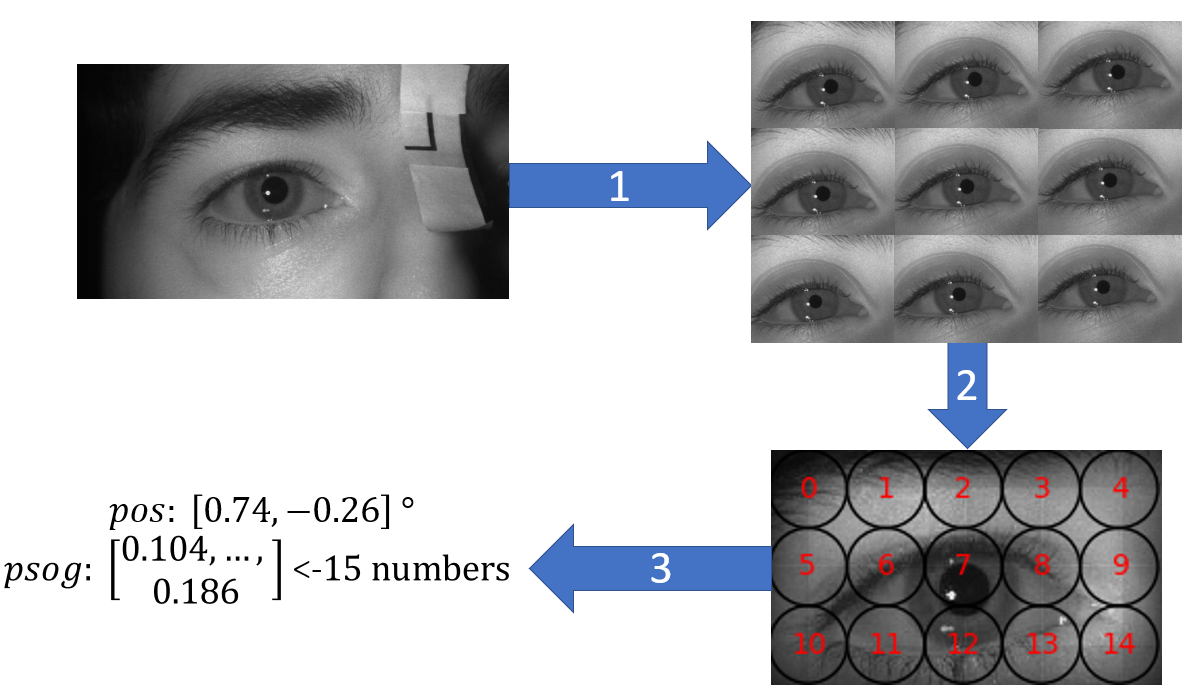
\includegraphics[width=0.47\textwidth]{preproc.png}
\end{center}
    \captionsetup{singlelinecheck=off}
   \caption{Preprocessing pipeline:
   \begin{enumerate}
        \item Account for head movements, then shift and crop.
       \item For each cropped image, simulate PSOG sensor output (for each detection window one standard deviation of the gaussian kernel is depicted).
       \item Save raw sensor output with corresponding eye gaze position.
   \end{enumerate}
   }
\label{fig:data_preproc}
\end{figure}

\pagebreak

\section{Results}\label{sec:results}

\subsection{Model selection}

To utilize available data during the grid search as much as possible, it was split into $75\%$ of train and $25\%$ validation sets, without test part. Architectures with the best performance on the validation set are:
\begin{itemize}
    \item Low-power, MLP: $Dense(\, 20\, )\, x\, 6$, $\leq0.076$ MFLOPS \footnote{The upper limit is provided due to the different number of components left after PCA for different subjects\label{mlp_note}} 
    \item Low-power CNN: $Conv2D(\, 4\, )\, x\, 4\: +\: Dense(\, 20\, )\, x\, 4$, $0.084$ MFLOPS
    \item High-power MLP: $Dense(\, 96\, )\, x\, 4$, $\leq3.835$ MFLOPS \footnotemark[\getrefnumber{mlp_note}]
    \item High-power CNN: $Conv2D(\, 4\, )\, x\, 1\: +\: Dense(\, 96\, )\, x\, 3$, $2.909$ MFLOPS
\end{itemize}
Layers names follow Keras' naming convention, here: \\ $Conv2D(\, D\, )\, x\, L$ means $L$ convolution layers in a row, each with $D$ filters; $Dense(\, N\, )\, x\, L$ means $L$ fully-connected layers in a row, each with $N$ neurons. Each architecture is visualized in Figure \ref{fig:all_archs}

\subsection{Training process details}

To explore variability in training performance with respect to initial condition, training was repeated $10$ times for random initial values. This was done since Keras does not allow users to achieve reproducible results by fixing a seed value. 
We use Adam with Nesterov momentum \cite{dozat2016incorporating} as the optimization algorithm, and mean-squared error as the loss function. The learning rate is set to $0.001$, epsilon to $10^{-8}$, and all other parameters to the default values. To prevent over-fitting, the early-stopping \cite{caruana2001overfitting} technique is used. The training process ends as soon as the validation loss is not improving for the specified number of steps (patience parameter in Keras). For the "fine-tune" approach, models are pre-trained with batch size of $2000$ and patience of $100$. Data is split into several batches as described in the \nameref{ssec:ml} subsection. Every batch is individually considered as the test set, with remaining data split into $80$\%/$20$\% for train and validation sets, respectively. For both the "fine-tune" approach and for the training "from scratch", batch size is set to $200$, and patience to $50$. The only available data to build a map between photosensors output and eye gaze of the specific subject is gathered during the calibration procedure. To resemble the small amount of such data, a $24$\%/$6$\%/$70$\% train, validation and test split is used for both approaches. Note that the spatial distribution of gaze locations for the train split is different from calibration data. The attempt to address this issue is made in the \nameref{sec:disc} section.

\subsection{Statistical results}

For the low-power setup, Figure \ref{fig:lp_avg} shows error bars that represents the mean and one standard deviation of the spatial accuracy obtained for 10 repetitions of training for each combination of architecture and approach for all subjects (for the high-power setup, the same is presented in Figure \ref{fig:hp_avg}).

As can be seen, the best spatial performance is $0.57$\textdegree{} and $0.67$\textdegree{} for the low-power and high-power setup respectively. This observation is supported by the paired comparisons in Table \ref{tab:lp_tab_2} (high-power: Table \ref{tab:hp_tab_2}). For both setups, it is achieved with CNN architecture retrained from scratch for each subject. Nevertheless, the performance of the fine-tune approach for CNN is relatively worse for about $5$\% for both setups.

In Table \ref{tab:lp_tab_1} we present F-tests of the effect of architecture, approach and their interaction for the low-power setup (high-power: Table \ref{tab:hp_tab_1}). The statistically significant interaction means that the effect of approach depends on the level of architecture and the effect of architecture depends on the level of approach. Table \ref{tab:lp_tab_2} presents the post-hoc paired comparisons for all combinations of architecture and approach for the low-power setup (high-power: Table \ref{tab:hp_tab_2}).  All $p$-values are adjusted for multiple comparisons.  All paired comparisons were statistically significant except for the comparison between MLP, approach "fine-tune" and CNN, approach "fine-tune". This effect is a statistical trend ($p = 0.07$). 

%% Lee's comment about plots
%   Means and SDs for each combination of Architeture and Approach.  Means are least-squared estimates. Note that the statistical tests are based on differences between these levels, adjusted for subject effects.  Therefore, different plots would be needed to illustrate each statistical result.

%%%%%%%%%%%%%%%%%%%%%%%%%%%%%%%%%%%%%%%%%%%
\begin{figure*}\centering
    \begin{subfigure}{.98\linewidth}
     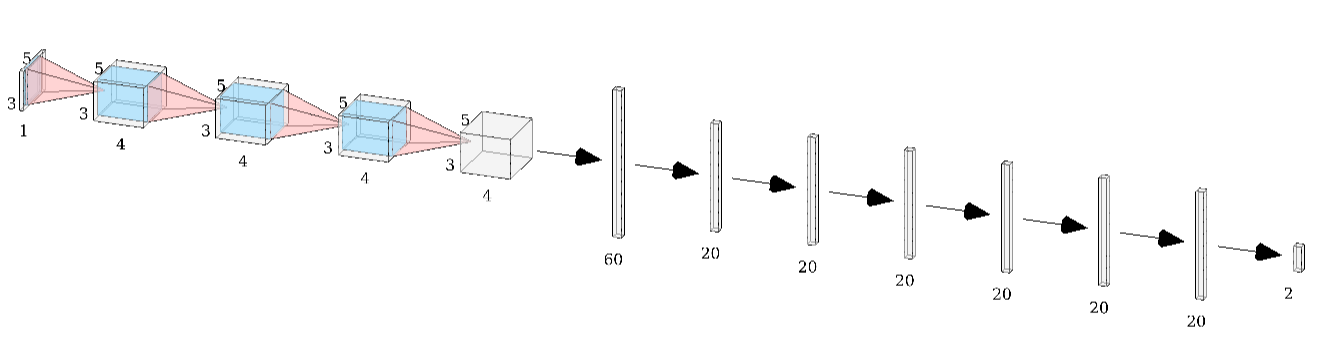
\includegraphics[width=0.98\linewidth]{lp_cnn_arch_crop.png}
        \caption{Low-power CNN}
    \end{subfigure}
    \begin{subfigure}{.74\linewidth}
     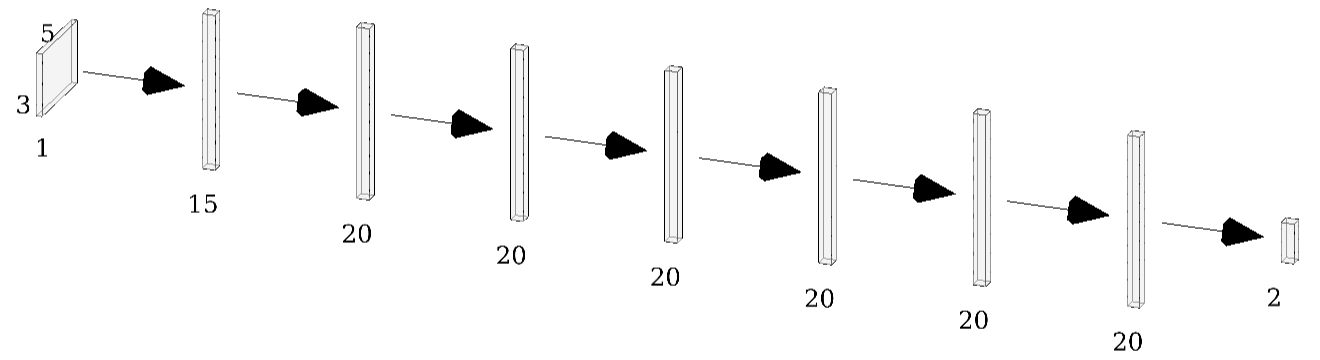
\includegraphics[width=0.98\linewidth]{lp_mlp_arch_crop.png}
        \caption{Low-power MLP}
    \end{subfigure}
    \begin{subfigure}{.49\linewidth}
     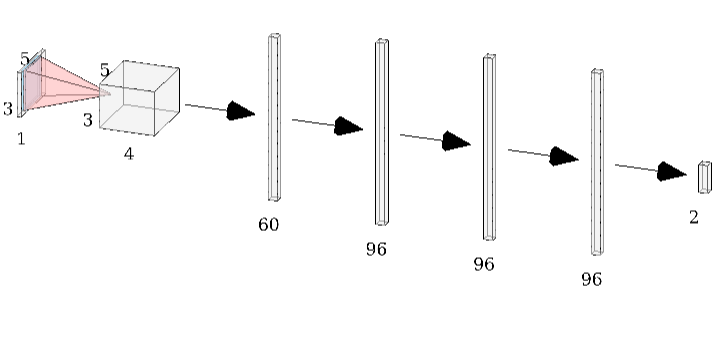
\includegraphics[width=0.98\linewidth]{hp_cnn_arch_crop.png}
        \caption{High-power CNN}
    \end{subfigure}
    \begin{subfigure}{.49\linewidth}
     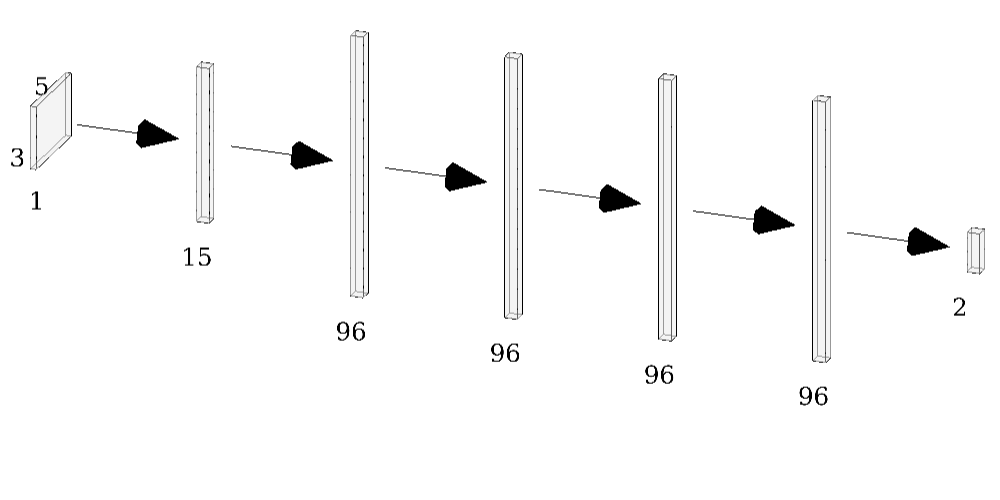
\includegraphics[width=0.98\linewidth]{hp_mlp_arch_crop.png}
        \caption{High-power MLP}
    \end{subfigure}
\caption{Neural network architectures used}
\label{fig:all_archs}
\end{figure*}
%%%%%%%%%%%%%%%%%%%%%%%%%%%%%%%%%%%%%%%%%%%

%% High-power, error bars

\begin{figure}[h!]
\begin{center}
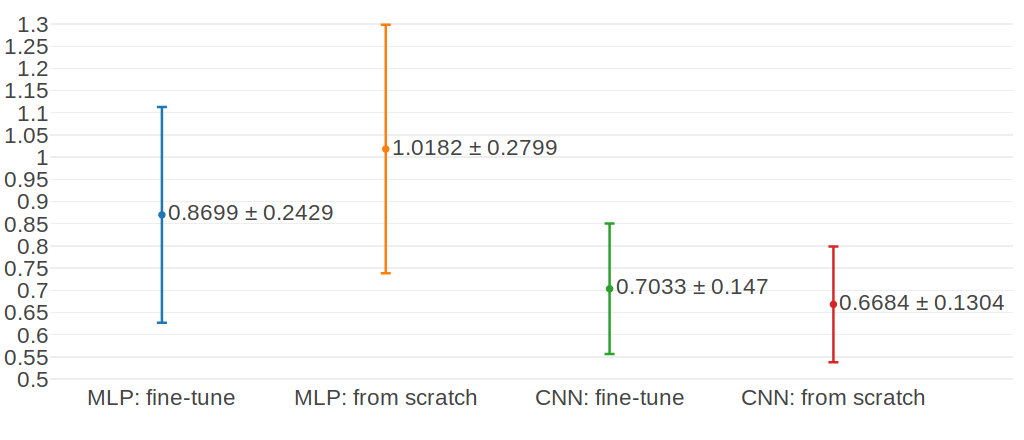
\includegraphics[width=0.47\textwidth]{lp_avg_better_crop.png}
\end{center}
\caption{Low-power setup, spatial accuracy error bars}
\label{fig:lp_avg}
\end{figure}

% %% High-power, MLP

% \begin{figure}[h!]
% \begin{center}
% \includegraphics[width=0.5\textwidth]{hp_mlp_avg_crop.png}
% \end{center}
% \caption{High-power setup, box plots that represents spatial accuracy obtained for 10 repetitions of training for each approach for each subject for MLP architecture}
% \label{fig:hp_mlp}
% \end{figure}

% %% High-power, CNN

% \begin{figure}[h]
% \begin{center}
% \includegraphics[width=0.5\textwidth]{hp_cnn_avg_crop.png}
% \end{center}
% \caption{High-power setup, box plots that represents spatial accuracy obtained for 10 repetitions of training for each approach for each subject for CNN architecture}
% \label{fig:hp_cnn}
% \end{figure}

\begin{table}[h]
    \caption{Low-power setup, statistical analysis}
	\begin{subtable}[h]{0.47\textwidth}
	    \centering
	    \caption{Tests of Fixed Effects}
	    \begin{adjustbox}{max width=0.6\columnwidth}
		\begin{tabular}{>{\columncolor[rgb]{0.93,0.95,0.98}}cllll}
        \toprule
        \rowcolor[rgb]{0.93,0.95,0.98}
            \color[rgb]{0.07,0.13,0.47}\textbf{Effect} &
            \color[rgb]{0.07,0.13,0.47}\textbf{Num DF} &
            \color[rgb]{0.07,0.13,0.47}\textbf{Den DF} &
            \color[rgb]{0.07,0.13,0.47}\textbf{F Value} &
            \color[rgb]{0.07,0.13,0.47}\textbf{Pr > F} \\
        \midrule
        arch           & 1 & 32.4 & 17.22 & 0.0002 \\
        \midrule
        appr           & 1 & 834 & 212.14 & \textless{}.0001 \\
        \midrule
        arch*appr           & 1 & 834 & 554.98 & \textless{}.0001 \\
        \bottomrule
        \end{tabular}
		\end{adjustbox}
	
	\label{tab:lp_tab_1}
	\end{subtable}
	\hfill

	\begin{subtable}[h]{0.47\textwidth}
		\centering
		\caption{Differences of LS Means}
		\begin{adjustbox}{max width=\columnwidth}
		\begin{tabular}{>{\columncolor[rgb]{0.93,0.95,0.98}}ccclllll}
        \toprule
        \rowcolor[rgb]{0.93,0.95,0.98}
            \color[rgb]{0.07,0.13,0.47}\textbf{\textnumero} & \color[rgb]{0.07,0.13,0.47}\textbf{Group A} &
            \color[rgb]{0.07,0.13,0.47}\textbf{Group B} &
            \color[rgb]{0.07,0.13,0.47}\textbf{Estimate} &
            \color[rgb]{0.07,0.13,0.47}\textbf{Standard Error} &
            \color[rgb]{0.07,0.13,0.47}\textbf{DF} &
            \color[rgb]{0.07,0.13,0.47}\textbf{t Value} &
            \color[rgb]{0.07,0.13,0.47}\textbf{Adj P} \\
        \midrule
        1           & 1       & 2       & -0.1483 & 0.005500       & 834  & -26.96  & \textless{}.0001  \\
        \midrule
        2           & 1       & 3       & 0.1666   & 0.06234        & 32.7 & 2.67    & 0.0683           \\
        \midrule
        3           & 1       & 4       & 0.2016   & 0.06234        & 32.7 & 3.23    & 0.0155            \\
        \midrule
        4           & 2       & 3       & 0.3149   & 0.06234        & 32.7 & 5.05    & \textless{}.0001   \\
        \midrule
        5           & 2       & 4       & 0.3498   & 0.06234        & 32.7 & 5.61    & \textless{}.0001  \\
        \midrule
        6           & 3       & 4       & 0.03498  & 0.005500       & 834  & 6.36    & \textless{}.0001 \\
        \bottomrule
        \end{tabular}
        
	\end{adjustbox}
		
		\label{tab:lp_tab_2}
	\end{subtable}
	
	\label{tab:lp_tab}
\end{table}

% %% Low-power, MLP

% \begin{figure}[h]
% \begin{center}
% \includegraphics[width=0.5\textwidth]{lp_mlp_avg_crop.png}
% \end{center}
% \caption{Low-power setup, box plots that represents spatial accuracy obtained for 10 repetitions of training for each approach for each subject for MLP architecture}
% \label{fig:lp_mlp}
% \end{figure}

% %% Low-power, CNN

% \begin{figure}[h]
% \begin{center}
% \includegraphics[width=0.5\textwidth]{lp_cnn_avg_crop.png}
% \end{center}
% \caption{Low-power setup, box plots that represents spatial accuracy obtained for 10 repetitions of training for each approach for each subject for CNN architecture}
% \label{fig:lp_cnn}
% \end{figure}

\begin{table}[h]
    \caption{High-power setup, statistical analysis}
	\begin{subtable}[h]{0.47\textwidth}
	    \centering
	    \caption{Tests of Fixed Effects}
	    \begin{adjustbox}{max width=0.6\columnwidth}
		\begin{tabular}{>{\columncolor[rgb]{0.93,0.95,0.98}}cllll}
        \toprule
        \rowcolor[rgb]{0.93,0.95,0.98}
            \color[rgb]{0.07,0.13,0.47}\textbf{Effect} &
            \color[rgb]{0.07,0.13,0.47}\textbf{Num DF} &
            \color[rgb]{0.07,0.13,0.47}\textbf{Den DF} &
            \color[rgb]{0.07,0.13,0.47}\textbf{F Value} &
            \color[rgb]{0.07,0.13,0.47}\textbf{Pr > F} \\
        \midrule
        arch           & 1 & 33.3 & 14.27 & 0.0006 \\
        \midrule
        appr           & 1 & 834 & 193.82 & \textless{}.0001 \\
        \midrule
        arch*appr           & 1 & 834 & 524.27 & \textless{}.0001 \\
        \bottomrule
        \end{tabular}
		\end{adjustbox}
	\label{tab:hp_tab_1}
	\end{subtable}
	\hfill

	\begin{subtable}[h]{0.47\textwidth}
		\centering
		\caption{Differences of LS Means}
		\begin{adjustbox}{max width=\columnwidth}
		\begin{tabular}{>{\columncolor[rgb]{0.93,0.95,0.98}}ccclllll}
        \toprule
        \rowcolor[rgb]{0.93,0.95,0.98}
            \color[rgb]{0.07,0.13,0.47}\textbf{\textnumero} & \color[rgb]{0.07,0.13,0.47}\textbf{Group A} &
            \color[rgb]{0.07,0.13,0.47}\textbf{Group B} &
            \color[rgb]{0.07,0.13,0.47}\textbf{Estimate} &
            \color[rgb]{0.07,0.13,0.47}\textbf{Standard Error} &
            \color[rgb]{0.07,0.13,0.47}\textbf{DF} &
            \color[rgb]{0.07,0.13,0.47}\textbf{t Value} &
            \color[rgb]{0.07,0.13,0.47}\textbf{Adj P} \\
        \midrule
        1           & 1       & 2       & -0.09301 & 0.003573       & 834  & -26.03  & \textless{}.0001  \\
        \midrule
        2           & 1       & 3       & 0.1408   & 0.05265        & 33.5 & 2.67    & 0.0680            \\
        \midrule
        3           & 1       & 4       & 0.1635   & 0.05265        & 33.5 & 3.10    & 0.0224            \\
        \midrule
        4           & 2       & 3       & 0.2338   & 0.05265        & 33.5 & 4.44    & 0.0002            \\
        \midrule
        5           & 2       & 4       & 0.2565   & 0.05265        & 33.5 & 4.87    & \textless{}.0001  \\
        \midrule
        6           & 3       & 4       & 0.02267  & 0.003573       & 834  & 6.35    & \textless{}.0001 \\
        \bottomrule
        \end{tabular}
        
	\end{adjustbox}
		
		\label{tab:hp_tab_2}
	\end{subtable}
	
	\label{tab:hp_tab}
\end{table}

%% Low-power, error bars

\begin{figure}[h!]
\begin{center}
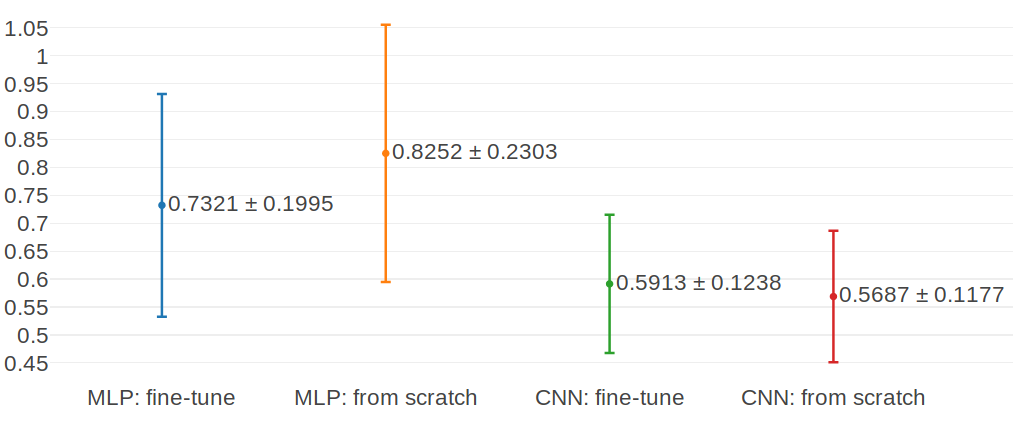
\includegraphics[width=0.47\textwidth]{hp_avg_better_crop.png}
\end{center}
\caption{High-power setup, spatial accuracy error bars}
\label{fig:hp_avg}
\end{figure}

\section{Discussion}\label{sec:disc}

\begin{table}[h]
    \centering
    \caption{Low-power setup, CNN training time analysis}
    \begin{adjustbox}{max width=\columnwidth}
	\begin{tabular}{>{\columncolor[rgb]{0.93,0.95,0.98}}cllll}
    \toprule
    \rowcolor[rgb]{0.93,0.95,0.98}
        \color[rgb]{0.07,0.13,0.47}\textbf{Batch size} &
        \color[rgb]{0.07,0.13,0.47}\textbf{Fine-tune (time/acc)} &
        \color[rgb]{0.07,0.13,0.47}\textbf{From scratch (time/acc)} \\
    \midrule
    200           & $96.45\pm{30.07} sec$ ($0.70\pm{0.15}$\textdegree{}) & $161.93\pm{44.88} sec$ ($0.67\pm{0.13}$\textdegree{}) \\
    \midrule
    2000           & $12.96\pm{5.61} sec$ ($1.01\pm{0.23}$\textdegree{}) & $33.27\pm{5.32} sec$ ($0.78\pm{0.15}$\textdegree{}) \\
    \bottomrule
    \end{tabular}
	\end{adjustbox}
\label{tab:tab_time_lp}
\end{table}

The time needed to enroll new user to a system is very important for a consumer-grade device. The most time-consuming part of our approach is model training on calibration data. Due to the non-efficient automatic garbage collector and hardware heating, the time spent for training is notably increasing over time for a long session of consecutive runs. It can be about $10$ times more at the end in comparison to the beginning. Therefore, we are not able to use information saved during our main evaluation. Then we train CNN architecture of the low-power setup only one time for each subject for two values of batch size: $200$ and $2000$. Means ($\pm{}$ one standard deviation) of resulting time and accuracy for both values are listed in Table \ref{tab:tab_time_lp}. It can be seen that a higher batch size can drastically improve training time but on the cost of decreased spatial accuracy. Despite training from scratch being more accurate, it is up to $2.5$ times slower, so \textbf{we pick fine-tune approach as the best} overall one. The proper evaluation of time complexity on actual hardware with possible optimizations applied should be done in the future work. 

Our work has following limitations: sensor shifts simulated by cropping, simulated photosensors output, and a random split of the whole recording into train and test set. While the first two should give a close approximation to results obtained using actual hardware, the later one does not reflect a real-case scenario where only calibration data is available to train on. Unfortunately, the custom eye-tracker did not allow us to obtain the eye-position signal from the calibration step. Fortunately, the grid of points used as stimuli for the random saccades task contains a subset similar to the calibration grid. We decided to exploit this observation, training the model only on samples that have euclidean distance no more than $35$ pixels from any point from the "calibration" grid (points $1, 3, 5, 9, 11, 13, 17, 19, 21$ on Figure \ref{fig:data_calib_split}). For most subjects, the data is unevenly spread around "calibration" points, providing very limited coverage for some of them (an example of such data is depicted in Figure \ref{fig:data_calib_bad}. At the same time, for some subjects the distribution is much better, as can be seen in Figure \ref{fig:data_calib_good}. This limitation cannot be fixed using an increased distance threshold, as it will lead to more points being added that were not fixations of interest. To get more reliable results, proper calibration data should be collected.

As was stated in the \nameref{sec:intro}, eye-tracking has a lot of potential applications in VR. Our study demonstrates adequate accuracy at sufficiently low power consumption to support general touchless interaction. However, it is still not clear how well this approach preserves specific features in the eye-signal that are essential for biometrics and health assessment.

Future work will require assembling real hardware to test the real-world validity of the proposed technique. This step is essential for developing power-efficient eye tracking sensors for VR headsets.

\begin{figure}[h]
    \centering
    \begin{subfigure}[h]{0.47\textwidth}
    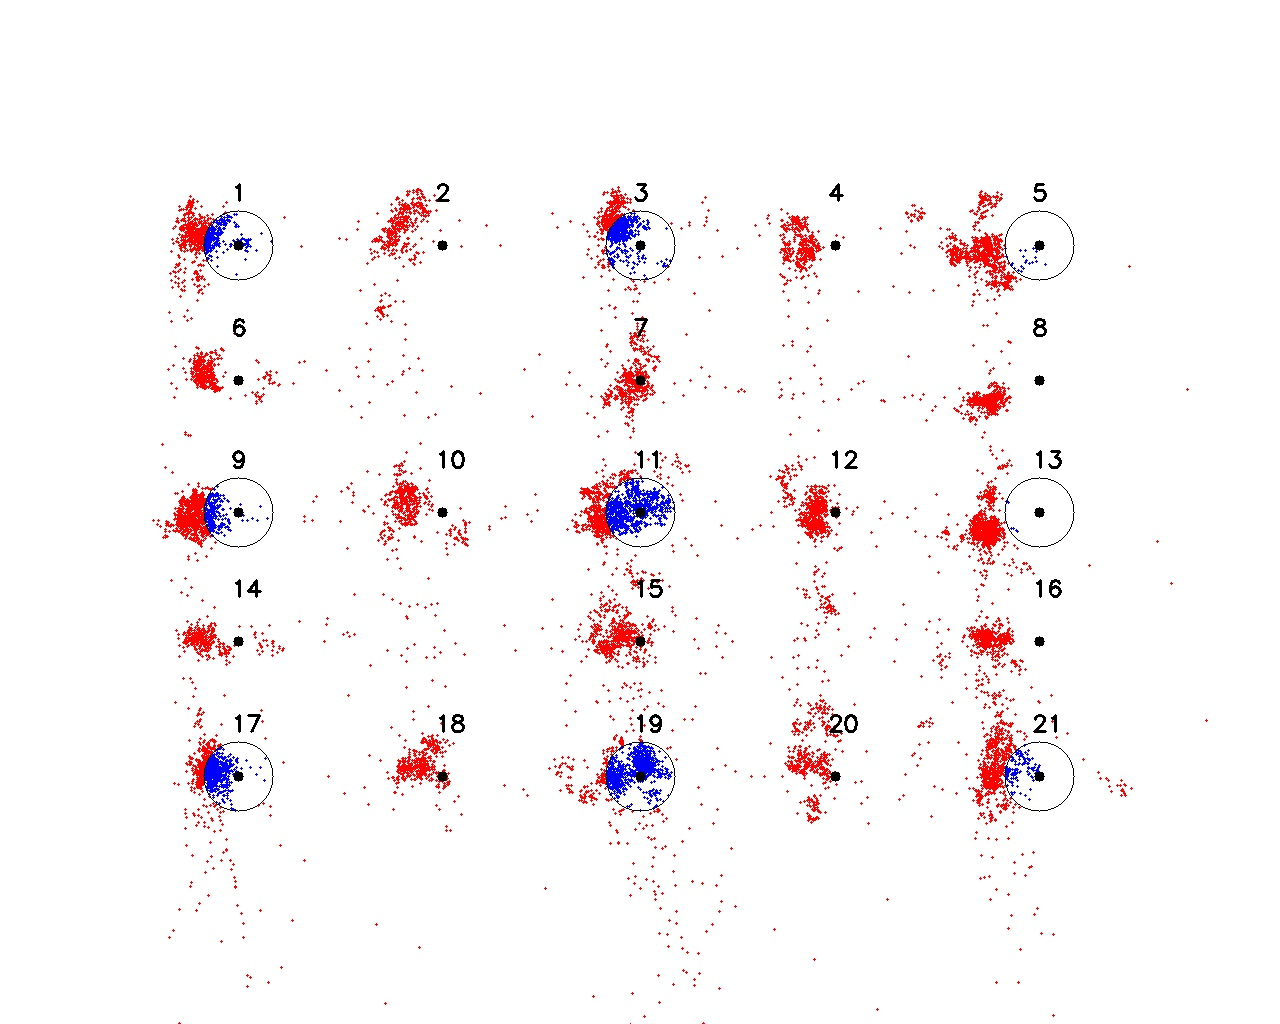
\includegraphics[width=\textwidth]{data_distrib_6_better.jpg}
    \captionsetup{singlelinecheck=off}
    \caption{Subject 6. Spatial accuracy on testing samples:
    \begin{enumerate}
        \item Low-power setup: $1.57$\textdegree{}
        \item High-power setup: $1.4$\textdegree{}
    \end{enumerate}
    }
    \label{fig:data_calib_bad}
    \end{subfigure}
    
    \centering
    \begin{subfigure}[h]{0.47\textwidth}
    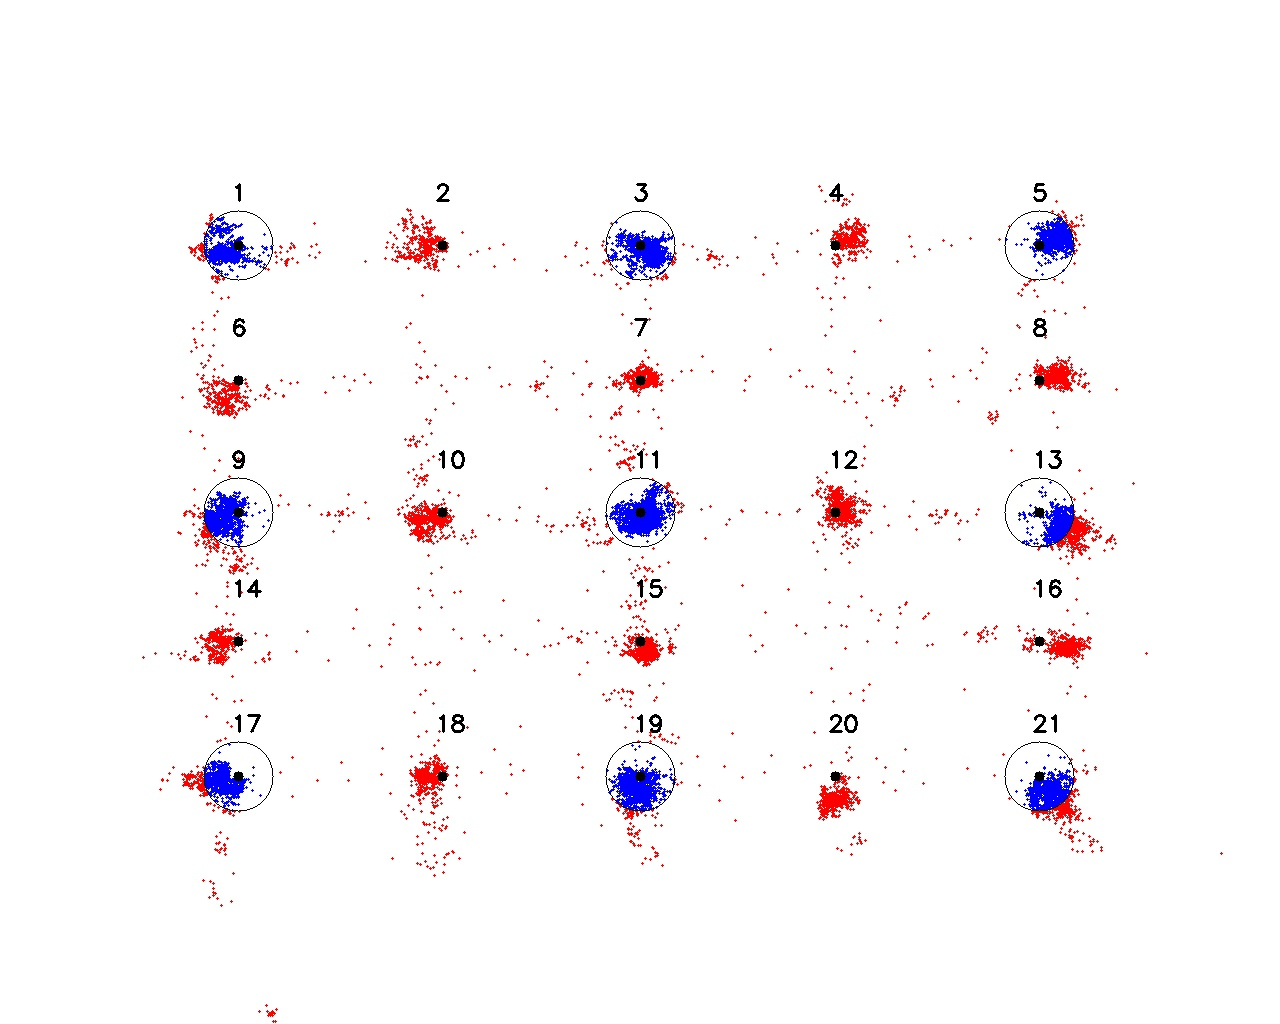
\includegraphics[width=\textwidth]{data_distrib_8_better.jpg}
        \captionsetup{singlelinecheck=off}
       \caption{Subject 8. Spatial accuracy on testing samples:
       \begin{enumerate}
            \item Low-power setup: $1.06$\textdegree{}
           \item High-power setup: $0.85$\textdegree{}
       \end{enumerate}
       }
    \label{fig:data_calib_good}
    \end{subfigure}
    \caption{Examples of: (\protect\subref{fig:data_calib_bad}) bad, (\protect\subref{fig:data_calib_good}) good split of data into blue training and red validation + testing samples that should reflect calibration procedure. Circles represents $35$px area around "calibration" points}
    \label{fig:data_calib_split}
\end{figure}

\section{Conclusion}

In this paper, we evaluated the PSOG-based eye-tracking sensor for portable VR headsets. Among all tested neural network architectures and approaches for calibrating the system to each new subject's eye traits, fine-tuning of convolution neural network works best. This combination was tested as two setups: with limited power consumption for embedded devices, and with no such restriction aiming for the best spatial accuracy.

The first setup can be used to implement the system on portable hardware platforms that already exist, with high sampling frequency of 1000 Hz and spatial accuracy of $0.7$\textdegree{}.
The second setup shows the potential of the proposed system for current wired hardware, because it maintains higher sampling frequency with better spatial accuracy of $0.59$\textdegree{}. Both setups are robust to sensor shifts. 

In summary, the proposed CNN architecture and fine-tuning training approach improved spatial accuracy and accelerated convergence versus benchmark techniques.

\begin{acks}

We thank Dr. Lee Friedman for his help with the statistical analysis part of the paper. 

\end{acks}

\bibliographystyle{ACM-Reference-Format}
%\bibliographystyle{unsrt}
\clearpage
\bibliography{references}

\end{document}
